\documentclass[12pt]{article}
\usepackage{float}
\usepackage{graphicx} 
\usepackage{mathtools}
\usepackage{amsmath, amsthm, amssymb}
\usepackage{siunitx} % SI Unit Functionality
\usepackage{times} % Times New Roman Font
\usepackage[symbols,americanvoltages]{circuitikz}%Circuit Illustration Package
\usepackage{steinmetz} %allows use of \phasor
\lefthyphenmin=5 %STOP HYPHENATING SMALL WORDS
\usepackage[toc,page]{appendix}

\title{\huge\bfseries Three Phase Open Loop Configuration PWM Generator for Use in Low Speed BLDC Control
}
\author{
  \\
  \\
  \\
  \huge Santos, Matthew\\
  \\
  \texttt{\huge 103103503}
  \and
  \\
  \\
  \\
  \huge Schulz, Kurtis\\
  \\
  \texttt{\huge 104077177}
}
\date{\phantom\\
    \phantom\\
    \phantom\\
    \phantom\\
    \phantom\\
    \phantom\\
    \phantom\\
    \phantom\\
    {\scshape\Large University Of Windsor}\\
    \phantom\\
    {\Large\itshape Department of Computer and Electrical Engineering}\\
    \phantom\\
    \phantom\\
    \phantom\\
    \phantom\\
    Submitted March 18, 2016
}

\begin{document}
\begin{titlepage}
	\centering
	
\includegraphics[width=0.65\textwidth]{UW_Header.png}\par\vspace{1cm}

	{\huge\bfseries Three Phase Open Loop Configuration PWM Generator for Use in Low Speed BLDC Control\par}
	\vspace{1cm}
	{\scshape\Large 88-226-01: Electronics I\par}
	\vspace{1cm}
	{\scshape\Large Project Proposal \par}
	\vspace{1.5cm}

	\vspace{2cm}
	{\Large\itshape Department of Computer and Electrical Engineering\par}
	\vfill
	Attention to\par
	Dr.~Mitra \textsc{Mirhassani}

	\vfill

% Bottom of the page
	{\large March 18,2016\par}
\end{titlepage}


\maketitle

\pagebreak
\tableofcontents
\pagebreak
\section{Introduction}%done

Brushless DC motors commonly abbreviated as BLDC have become widely used throughout the world. They are considered to be one of the most desired types of motors due to their increased efficiency, longer lifetime, and precision control. %These features are a direct result of their ability to achieve commutation through the controlled toggling of their supply currents as opposed to a dependence on mechanical commutation techniques.
In order to actuate a BLDC, an advanced pulse width modulation based control circuit is needed to correctly toggle the associated supply currents in the proper sequence. The vast majority of these control circuits operate using positioning feedback in order to properly synchronize commutation events. In order to account for this feedback requirement some motors are pre-built with position sensors (hall sensors) and the others are sensorless and typically controlled through the measure of back-EMF current. While proven to be adequate at high speeds, the sensorless technique fails at low RPM due to negligible back-emf and an open loop configuration with no feedback is required to control the motor.

\section{Proposal}

\subsection{Objective}%done

A customer has requested an open loop BLDC speed controller capable of operating a three phase "EMAX Model 2213-935kV" at 12V in the low to 500RPM region for use evaluating its slipping potential. Thus the objective of this project is to design and build a circuit capable of producing the pulse width modulation signals needed to operate the three phase BLDC motor as indicated. In addition the overall design of the controller is to requested to be modular in nature to allow for easy reconfiguration into a synchronous AC motor PWM controller.

\subsection{Implementation Strategy}

Following a \emph{considerable} amount of research and through examination of the BLDC in question a hybrid approach was taken whereby pulse signals are produced in a manner similar to sine wave pulse width modulation (SPWM) using comparators to reference sine waves produced in a Wien Bridge Oscillator to a known potential. This provided the added benefit of automatically allowing for a switching delay and easily allowing for the transition to AC motor control by simply changing the reference voltage to that of a triangular waveform (sine-triangular PWM generation). Furthermore to allow for strength control of the motor an additional layer of pulse width modulation was superimposed using a 555 timer circuit specifically setup to produce triangular waveforms such that it could also be used in AC motor control if necessary. The output signals are then connected to a standard H-bridge driver specifically designed to withstand the 0.8A current draw required for motor operation. See appendix A for the appropriate circuit schematics. Note many components were selected with respect to current inventory rather then ideal values.

\subsubsection{Constraints, Variables, and Simulation Results}

Three overall control variables are needed to allow for adequate control of the BLDC: speed, strength, and switching delay. Each of these parameters have been setup to be varied through the use of variable resistors labeled $Rs$, $Ra$, and $Rd$ respectively. Additional information on specifications, tolerances, and associated outputs of these and other parameters can be found throughout the schematic diagrams and output plots located in the appendices.

\subsubsection{Required Components}

For the purposes of this project all passive components were deemed exempt from the overall budget along with a number of components included in the provided analogue parts kit. In addition the customer is supplying the motor and two dual variable power supplies for use in operating both the motor and control circuit. The remaining parts are estimated to cost approximately \$9.30 and are for the most part readily available. For a full breakdown of the required components and associated costs see Appendix C: Materials List.

\section{Conclusions}

\begin{enumerate}
    \item The proposed circuit has been thoroughly simulated and is expected to perform adequately in the specified range.
    \item Through the modification of the Sine wave reference signal and PWM connections to the H-bridge both AC and DC PWM configurations are possible.
\end{enumerate}

\pagebreak

\begin{appendices}
\pagebreak

\section{Circuit Schematics}

\subsection{Overall Circuit Schematic Diagram}
\begin{figure}[H]
\centering
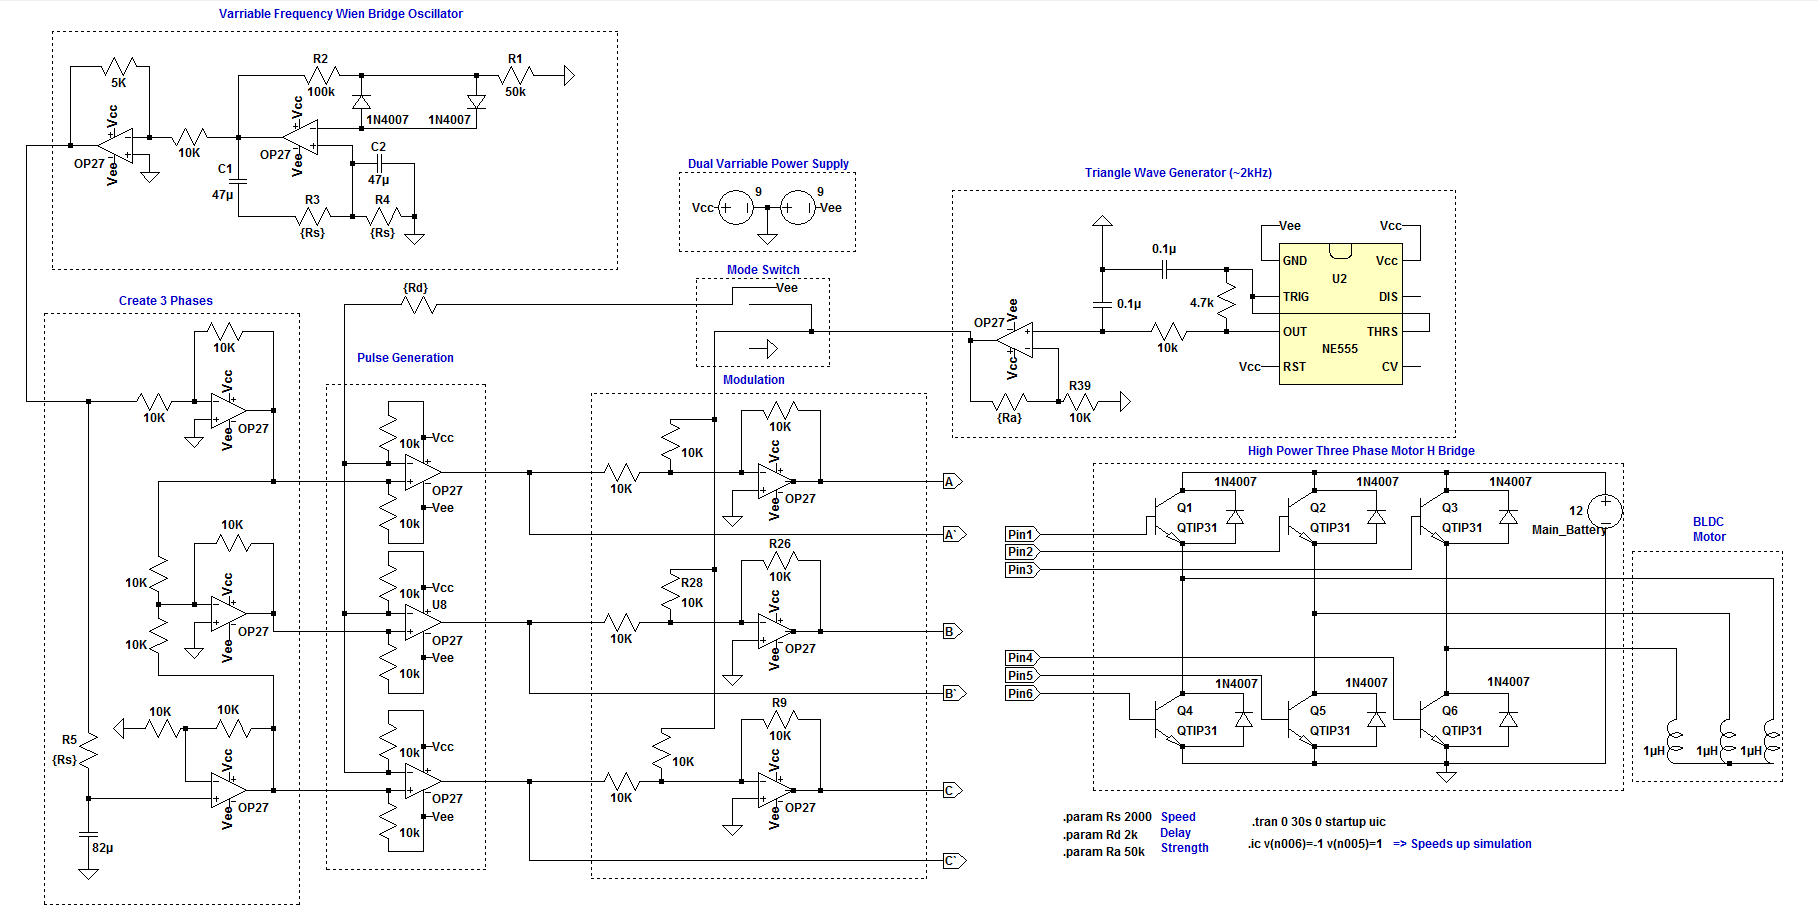
\includegraphics[scale=0.39,angle=90,origin=c]{Overal_General_Design.png}
\label{Overall_Design_V1}
\end{figure}
\subsection{AC Motor Controller Circuit Block Diagram}
\begin{figure}[H]
\centering
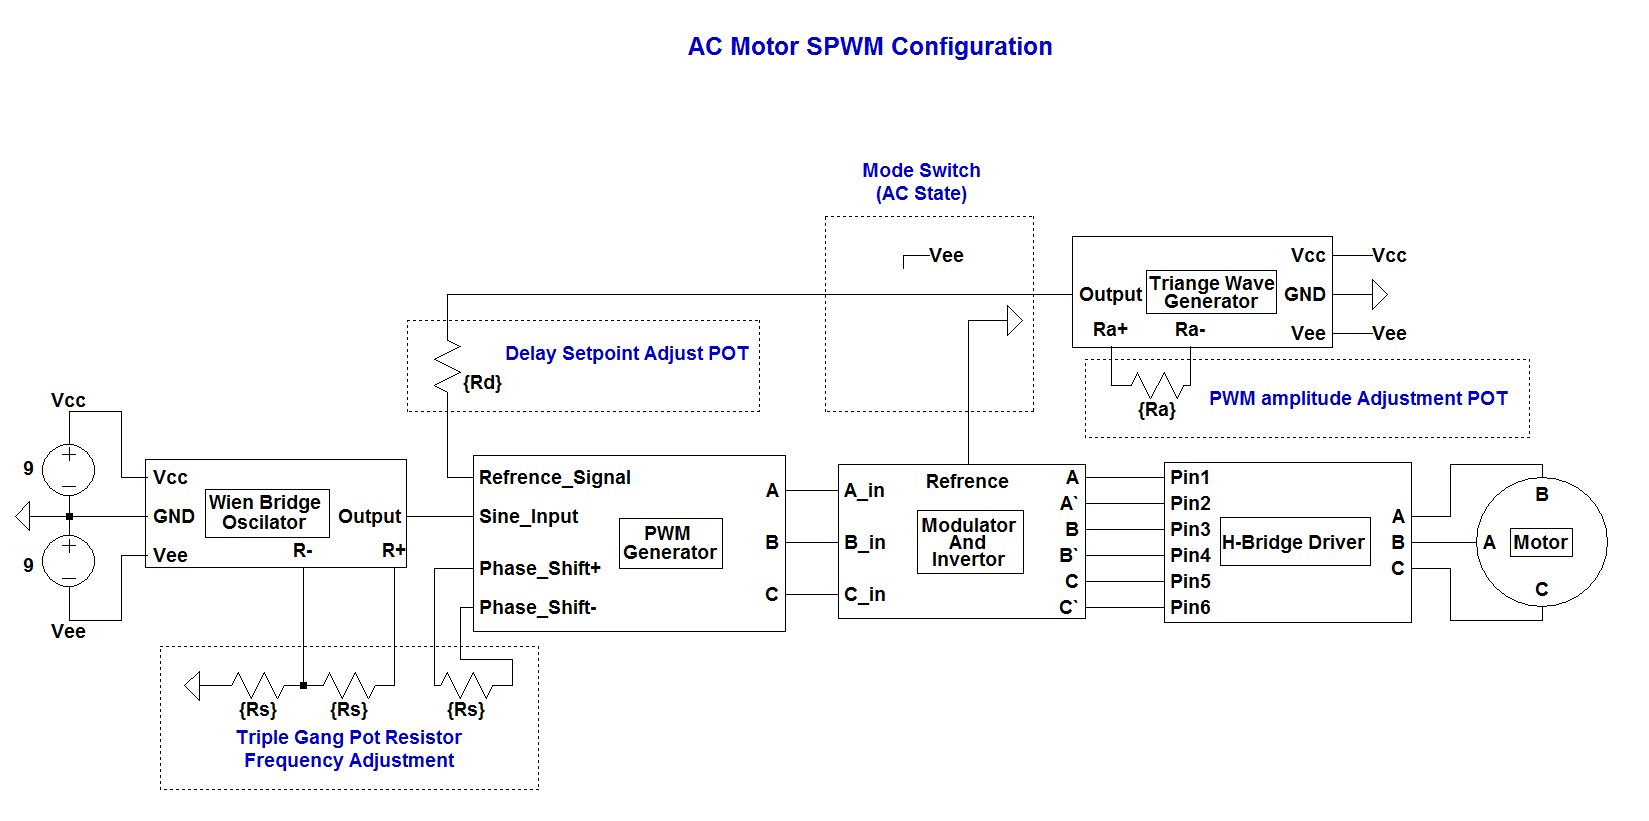
\includegraphics[scale=0.4,angle=90,origin=c]{AC_Block_Diagram.png}
\label{Overall_Design_V1}
\end{figure}
\subsection{DC Motor Controller Circuit Block Diagram}
\begin{figure}[H]
\centering
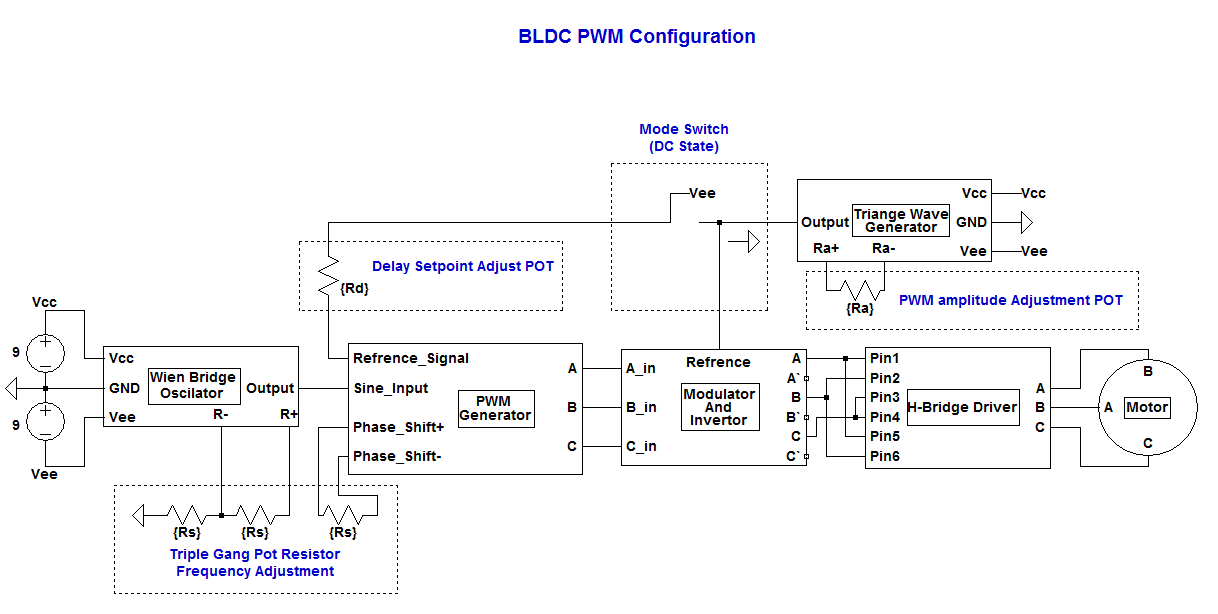
\includegraphics[scale=0.52,angle=90,origin=c]{DC_Block_Diagram.png}
\label{Overall_Design_V1}
\end{figure}
\subsection{Wien Bridge Oscillator Circuit}
\begin{figure}[H]
\centering
\includegraphics[scale=0.52,angle=90,origin=c]{Wien_Bridge_Oscillator.png}
\label{Overall_Design_V1}
\end{figure}
\subsection{Phase Generation Circuit}
\begin{figure}[H]
\centering
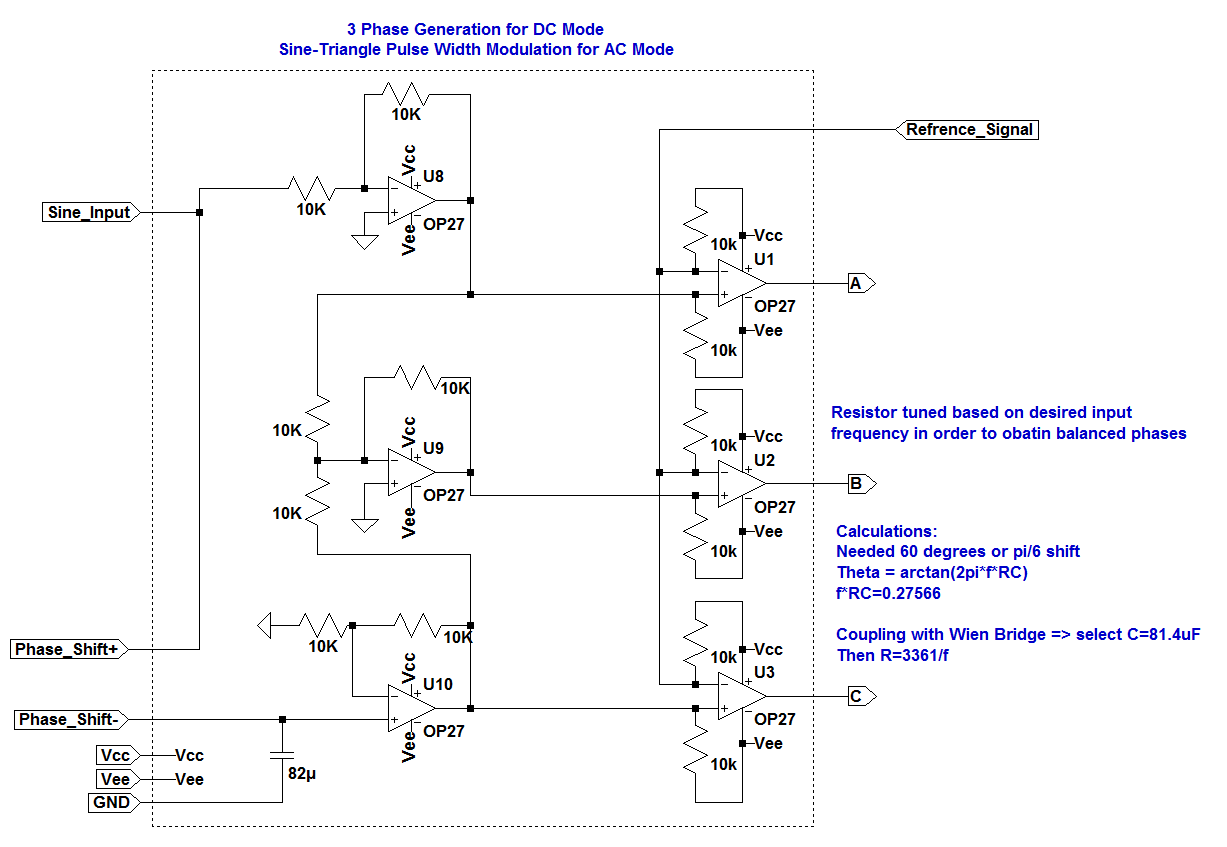
\includegraphics[scale=0.52,angle=90,origin=c]{Phase_Generation.png}
\label{Overall_Design_V1}
\end{figure}
\subsection{Modulation and Inversion Circuit}
\begin{figure}[H]
\centering
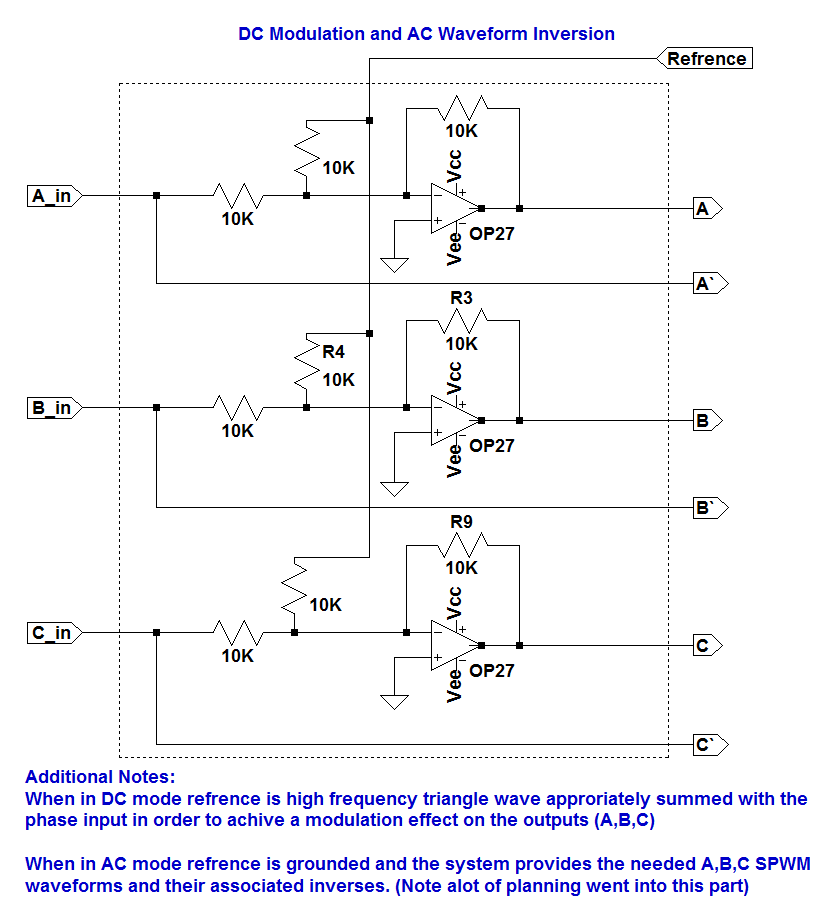
\includegraphics[scale=0.52,angle=90,origin=c]{Modulation_and_Inversion.png}
\label{Overall_Design_V1}
\end{figure}
\subsection{Triangle Wave Generator Circuit}
\begin{figure}[H]
\centering
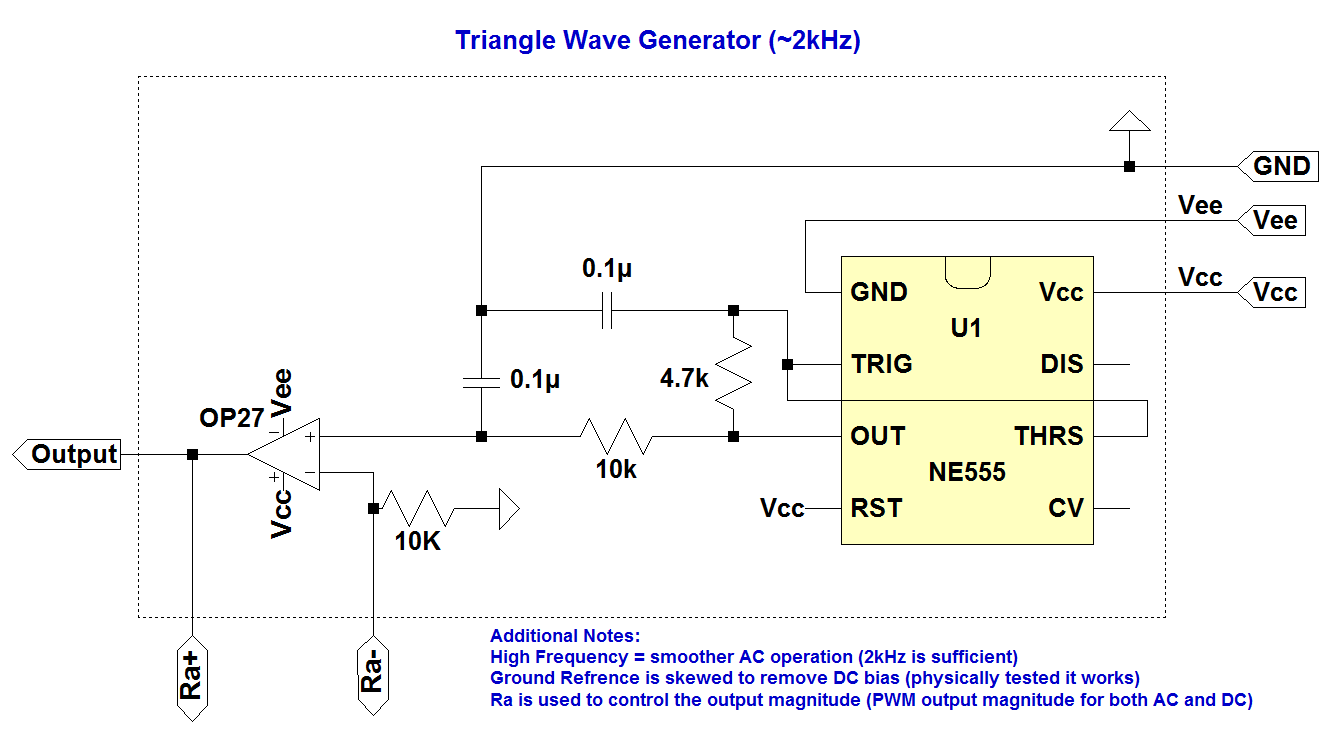
\includegraphics[scale=0.52,angle=90,origin=c]{Triangle_Wave_Generator.png}
\label{Overall_Design_V1}
\end{figure}
\subsection{H-Bridge Three Phase Driver Circuit}
\begin{figure}[H]
\centering
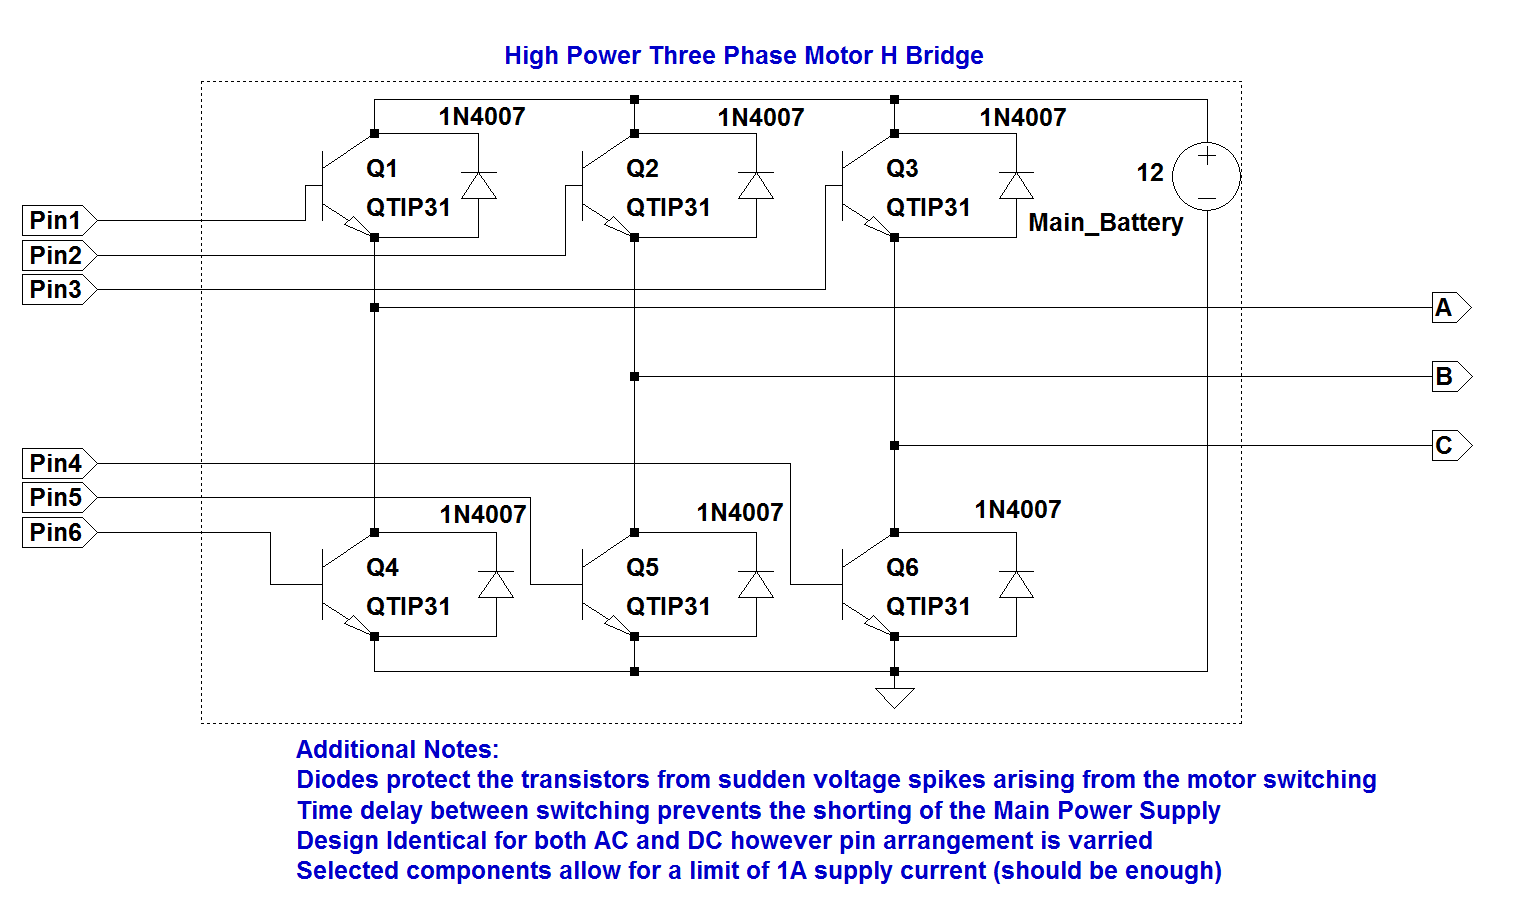
\includegraphics[scale=0.45,angle=90,origin=c]{H_bridge.png}
\label{Overall_Design_V1}
\end{figure}
\subsection{Simple Motor Model}
\begin{figure}[H]
\centering
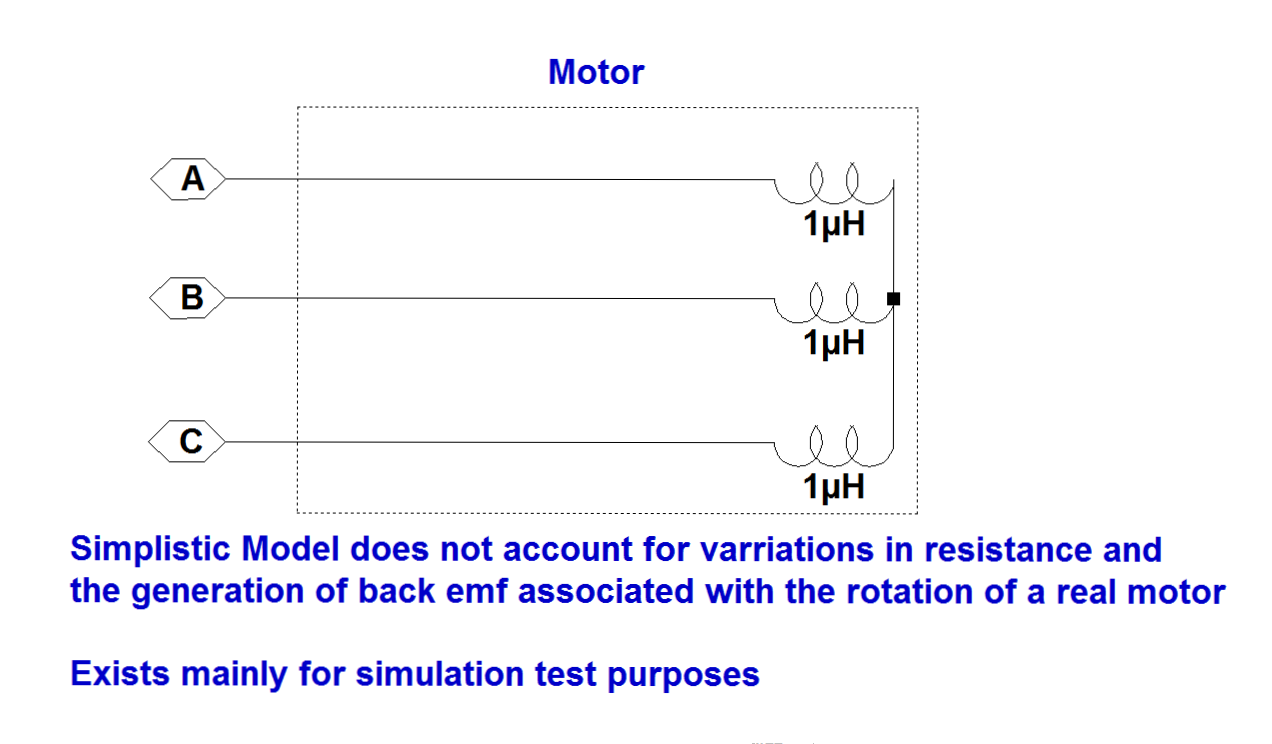
\includegraphics[scale=0.45,angle=90,origin=c]{Simple_Motor.png}
\label{Overall_Design_V1}
\end{figure}

\section{Simulation Results}

\subsection{Wien Bridge Oscillator Simulated Output}
\begin{figure}[H]
\centering
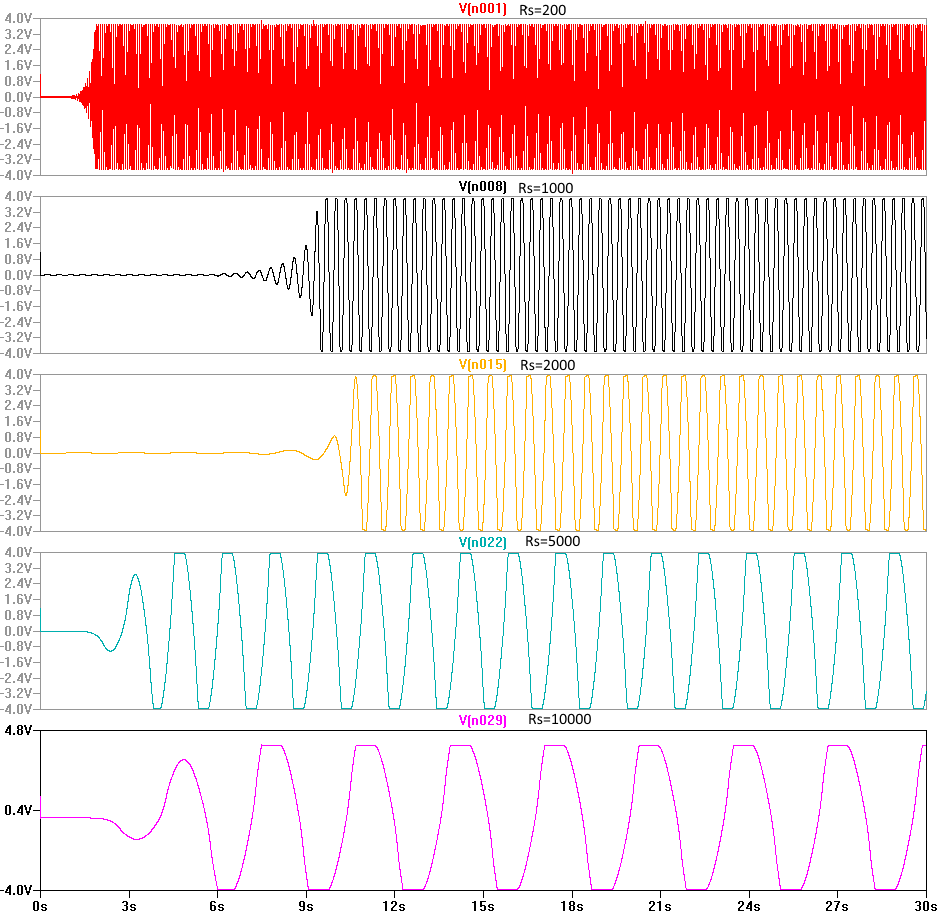
\includegraphics[scale=0.56,origin=c]{Wein_Bridge_Output.png}
\label{Triangle_Gen_Output}
\end{figure}
Thus it is shown that the adjustment of Rs correctly adjusts frequency output while maintaining overall magnitude. It is noted that the oscillations take time in order to reach saturation. Through the manipulation of Rs frequencies between 100Hz and 0.22Hz are incurred.

\subsection{Triangle Wave Generator Simulated Output}

\begin{figure}[H]
\centering
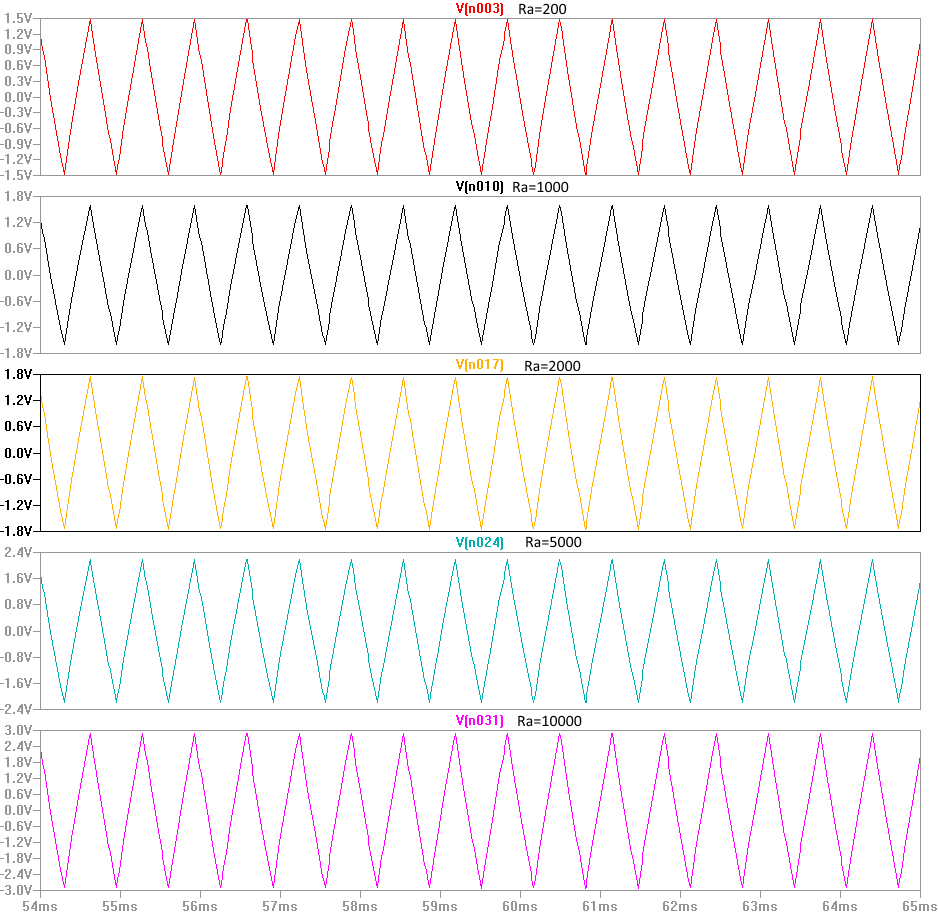
\includegraphics[scale=0.56,origin=c]{Triangle_Wave_Output.png}
\label{Triangle_Gen_Output}
\end{figure}
As expected the frequency output of the generator is fixed at approximately 1500Hz which should be sufficient for both Modulation of the DC control signal and sine wave resolution during the SPWM configuration.The varying of the Ra tuning resistor correctly adjusts the maximum output amplitude of the triangle wave from 1.5V to 3.0V as intended.

\subsection{Three Phase Sine Wave Generation}
\begin{figure}[H]
\centering
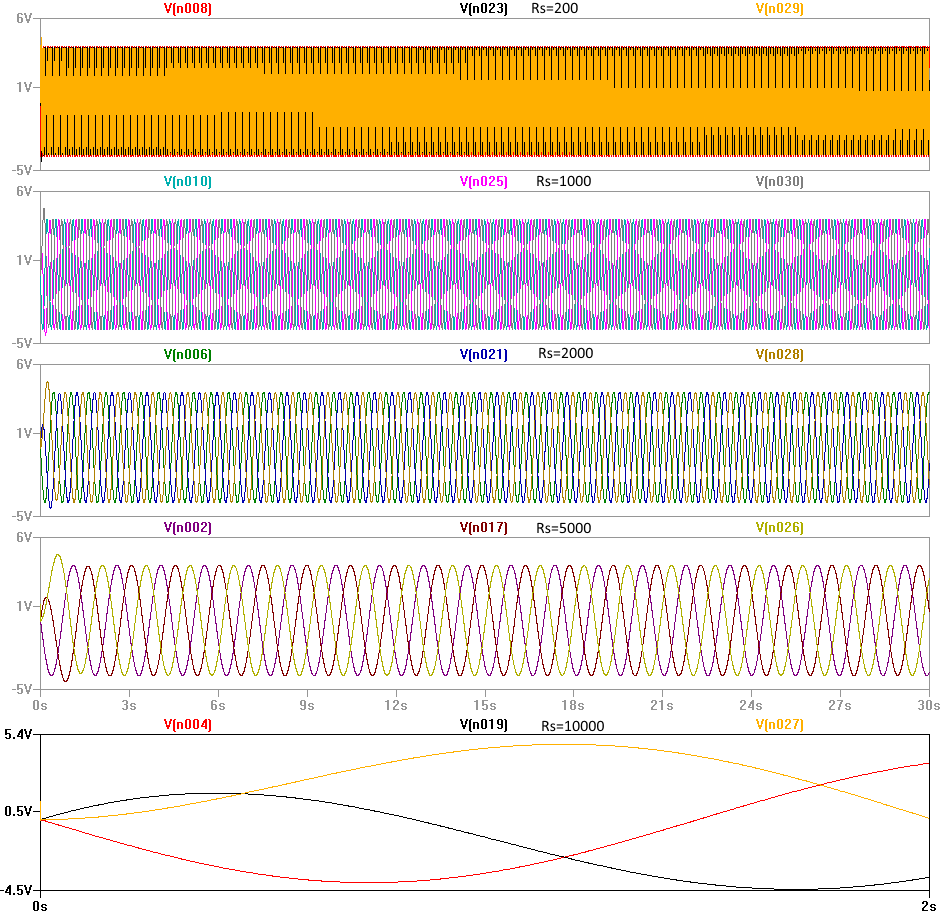
\includegraphics[scale=0.56,origin=c]{3_Phase_Output.png}
\label{Triangle_Gen_Output}
\end{figure}

Through the solving of the associated system of equations the phase shifting circuit was tuned in conjunction with the Wien Bridge oscillator frequency set-point so that it will correctly produce the required 120 degree shifts at any frequency as in the above simulation.

\subsection{Phase Generator Output (DC Configuration)}
\begin{figure}[H]
\centering
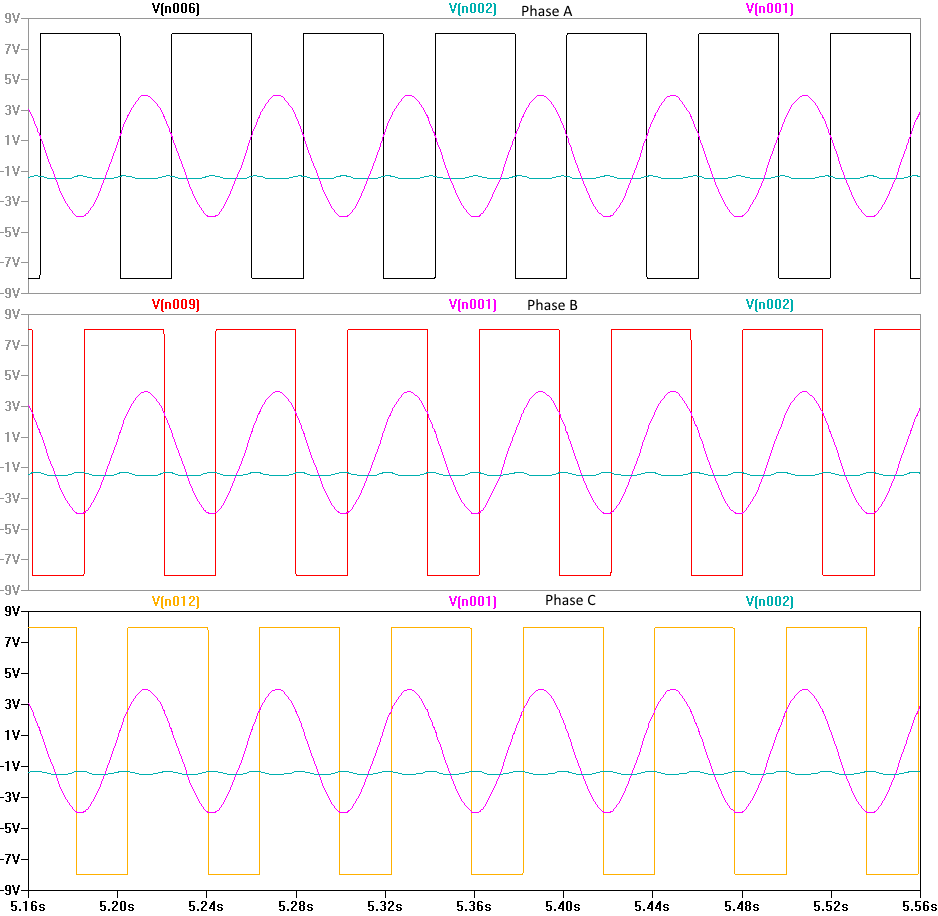
\includegraphics[scale=0.56,origin=c]{DC_Refrenced_Phase_Generation_Output.png}
\label{Triangle_Gen_Output}
\end{figure}

The above simulation illustrates the production of the \emph{inverse} ON/OFF switching signals needed for commutation switching (about to be fed into an inverting summer). As illustrated these square wave signals are produced by comparing the 3 phase sine waves with a DC setpoint established through the tuning of Rd. Through alteration of this Rd resistance the spacing between switching events is varied as evident in the next figure.

\begin{figure}[H]
\centering
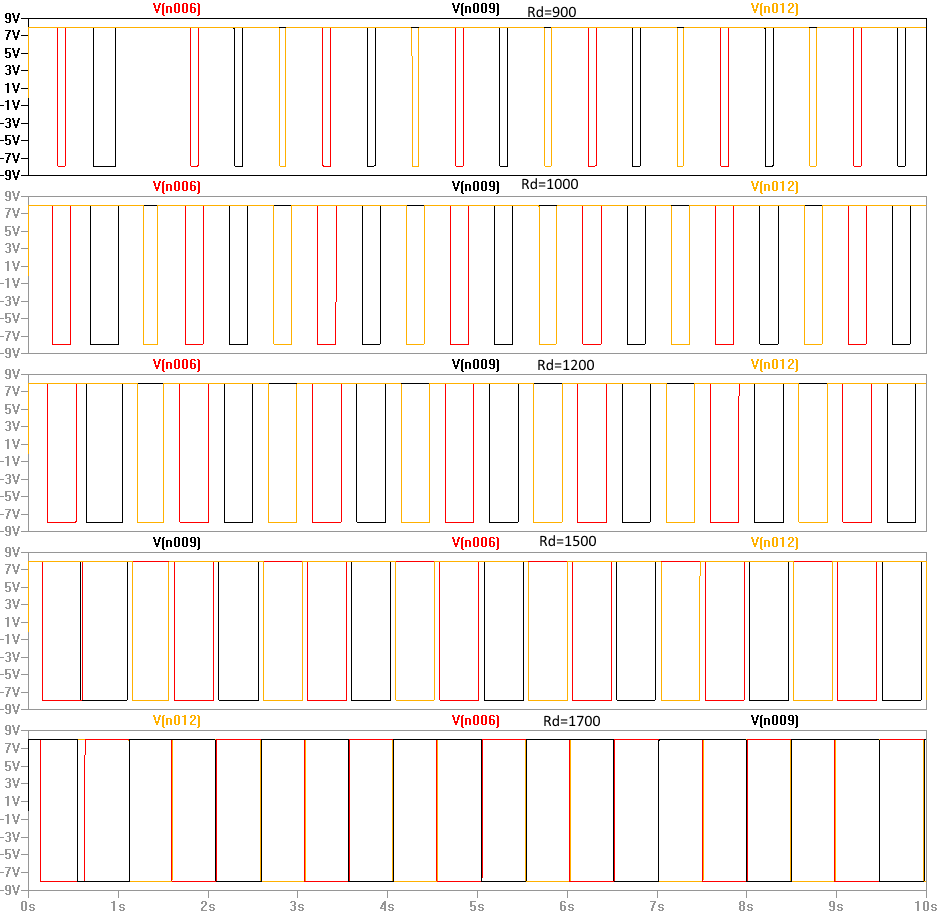
\includegraphics[scale=0.56,origin=c]{DC_Phase_Gen_Rd_Effect.png}
\label{Triangle_Gen_Output}
\end{figure}

From the figure it is clear to see that an increase in Rd produces shorter delay between actuation events. Care must be taken to always ensure a delay so as to prevent direct shorting of the H-Bridge driver. While not a variable of primary importance control of this delay allows for a smoothing like effect on motor control and also doubles as another form of modulation adjustment.

\subsection{Phase Generator Output (AC Configuration)}
\begin{figure}[H]
\centering
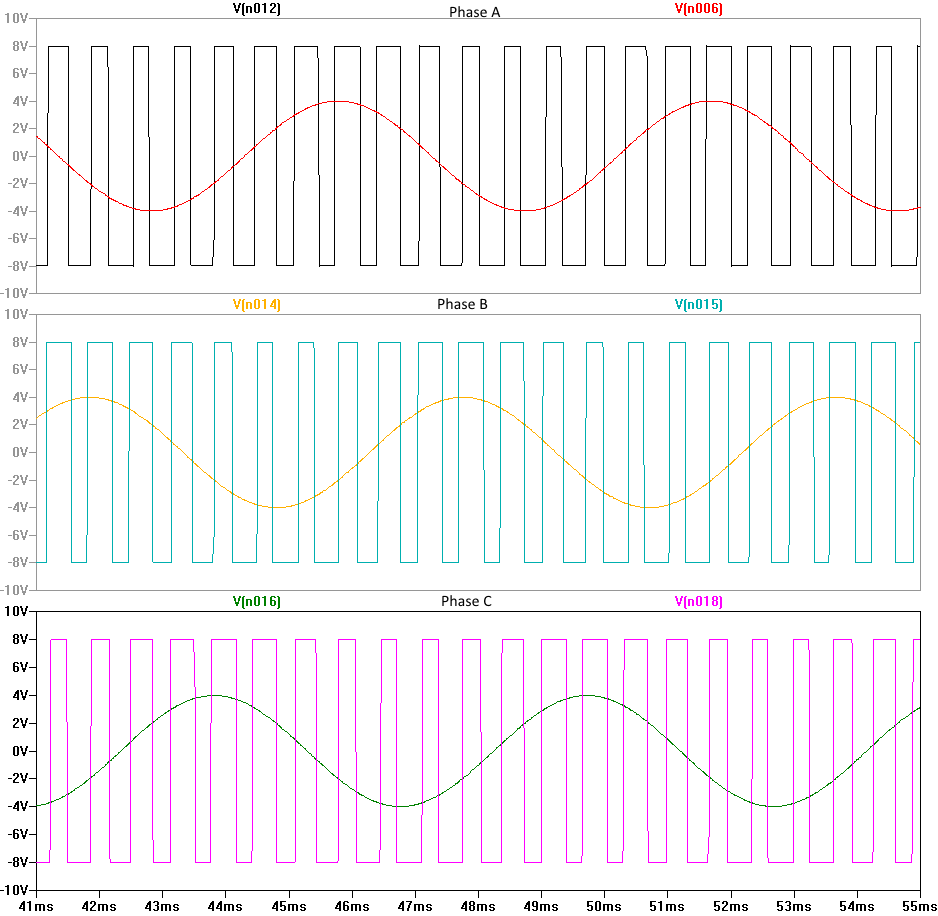
\includegraphics[scale=0.56,origin=c]{AC_Phase_Gen_Output.png}
\label{Triangle_Gen_Output}
\end{figure}

Through the toggling of a switch the triangular waveform is set to connect to the reference terminal of the Phase Generator Circuit and its previous connection is then grounded. The 3 phase sine wave is directly compared with a high frequency triangle wave which is used to directly approximate the sine wave in the form of Sinewave Pulse Width Modulation (SPWM). The results are illustrated above.  These three signals can be used to directly drive an AC motor however their inverse is also required and procured in the next stage

\subsection{Modulation and Inversion Output (DC Configuration)}
\begin{figure}[H]
\centering
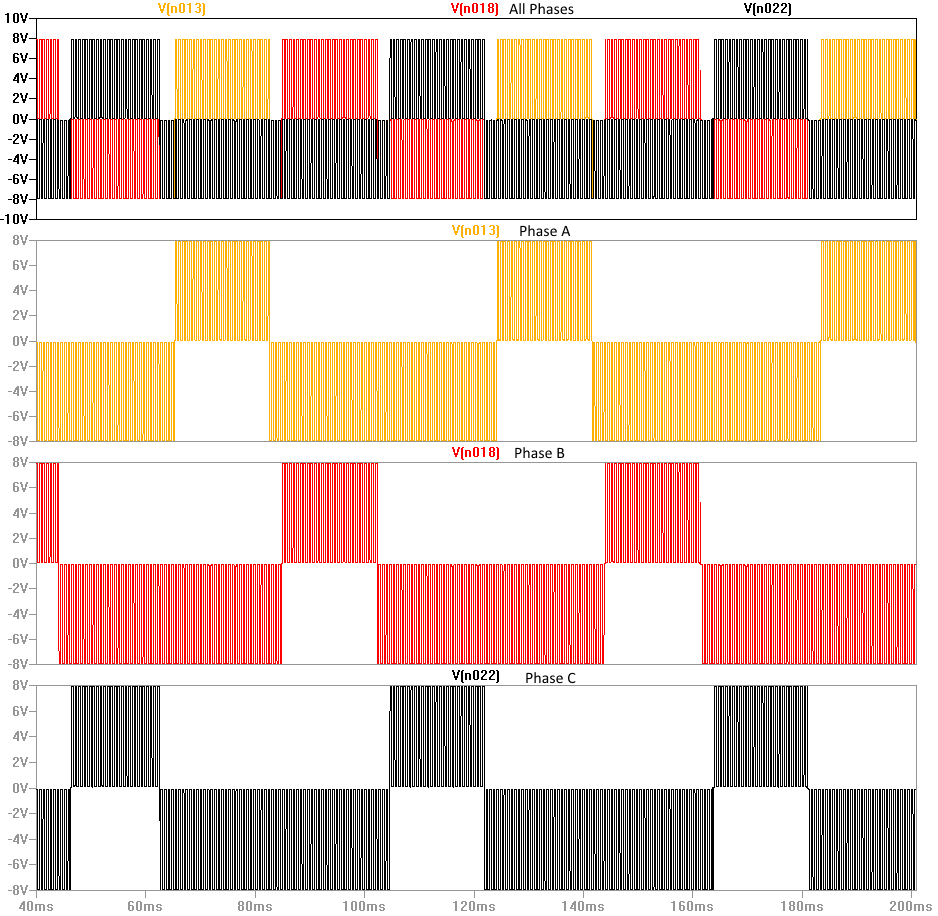
\includegraphics[scale=0.56,origin=c]{Modulation_Inversion_DC_Output_High_Modulation.png}
\label{Triangle_Gen_Output}
\end{figure}

In DC configuration this circuit acts as an inverting summer which superimposes the high frequency triangular waveform on top of the previously generated square wave pulse signals. This has a modulation effect and through the varying of Ra can be used to adjust the average strength of the signal entering the H-Bridge Driver as illustrated in the next figure.

\begin{figure}[H]
\centering
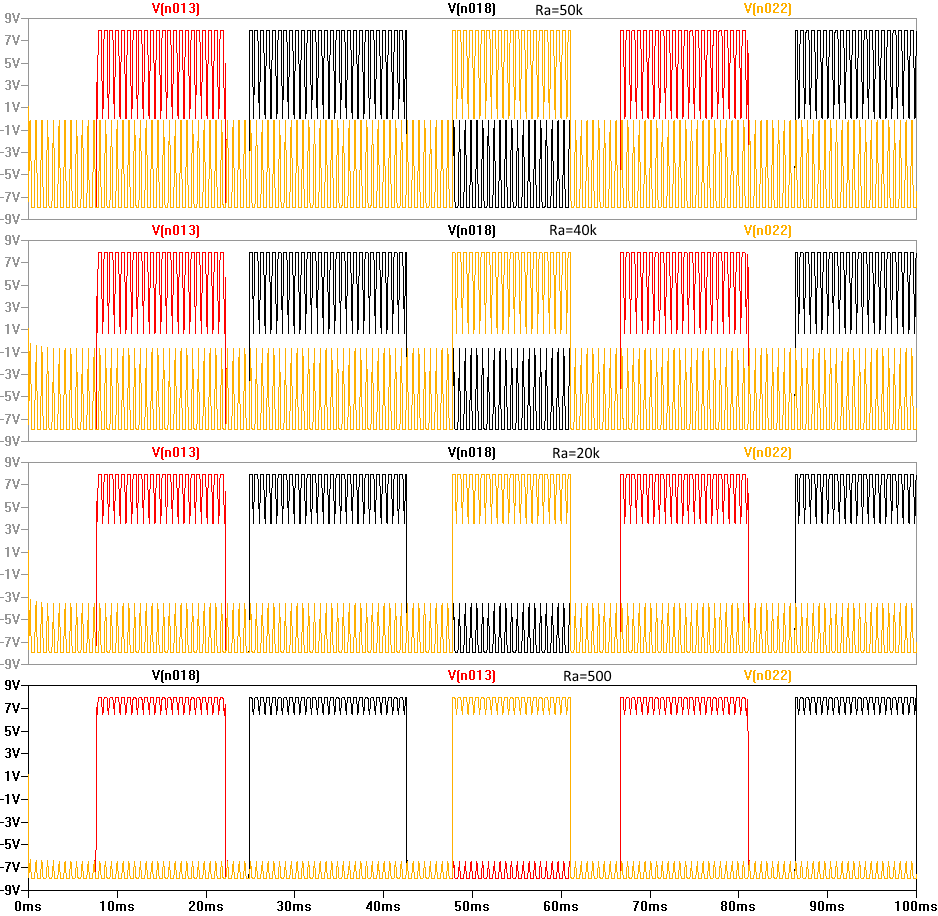
\includegraphics[scale=0.56,origin=c]{Modulation_Inversion_DC_Output_Varied_Modulation.png}
\label{Triangle_Gen_Output}
\end{figure}

As illustrated above the altering of Ra acts as a throthe on the output effectively adjusting its average amplitude through time based switching as per the definition of pulse width modulation.

\subsection{Modulation and Inversion Output (AC Configuration)}

\begin{figure}[H]
\centering
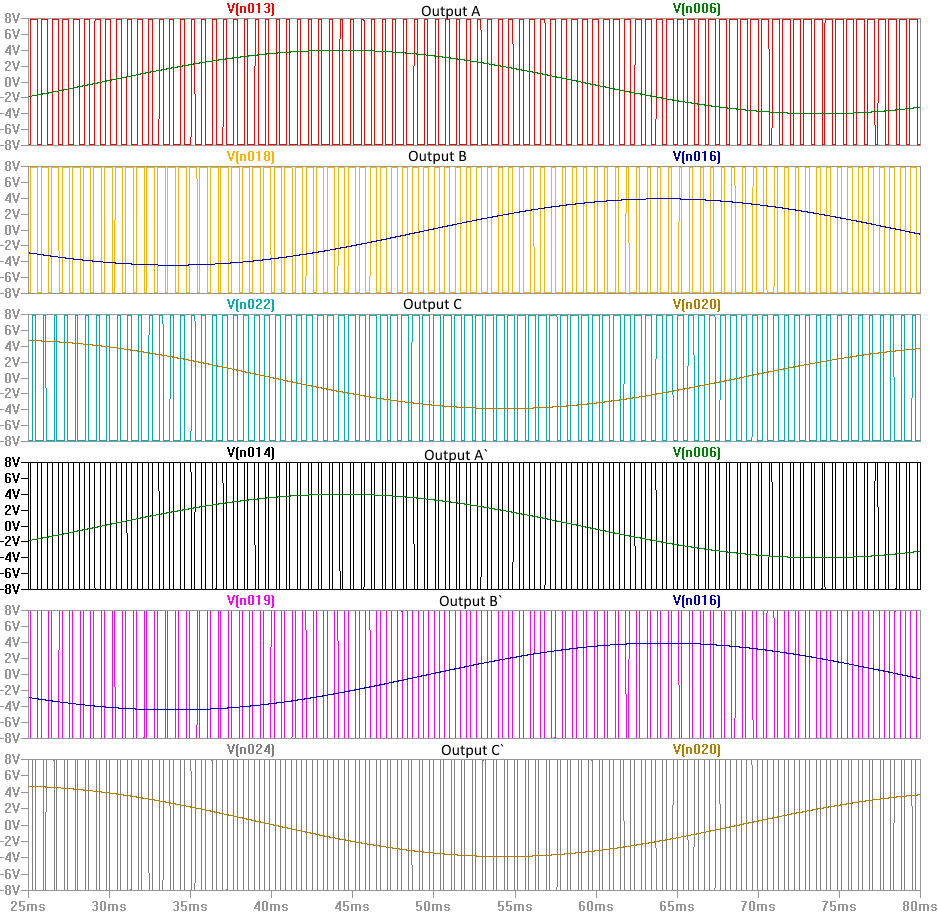
\includegraphics[scale=0.56,origin=c]{AC_PWM_FINAL.png}
\label{Triangle_Gen_Output}
\end{figure}


In this configuration the circuit is simply an inverter and is used to extract the required converse waveforms of the SPWM signals coming from the phase generator output. After inversion all the required signals for AC motor commutation have been produced and can be directly inserted into the H-bridge.

\subsection{Simulated Motor Current Waveforms}

In order to verify that the controller operates correctly the current waveforms in each of the windings were directly measured for DC configuration and the results are shown below.

\begin{figure}[H]
\centering
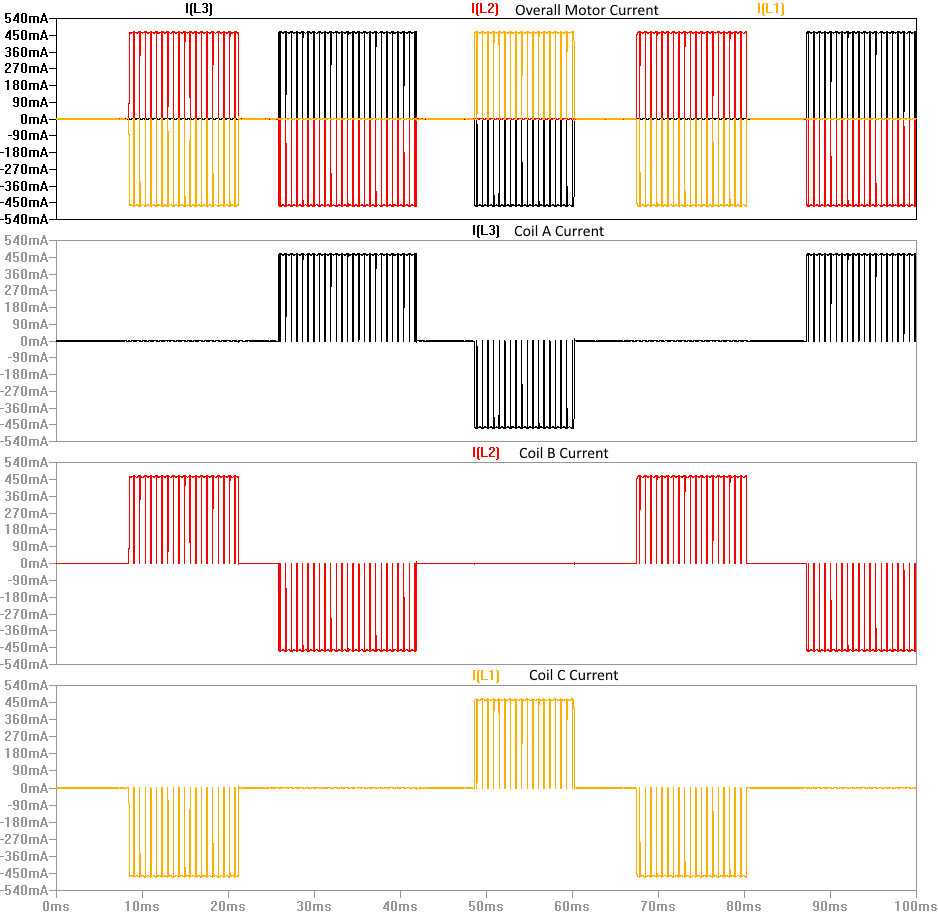
\includegraphics[scale=0.56,origin=c]{Motor_OUTPUT_DC.png}
\label{Triangle_Gen_Output}
\end{figure}

From the figure it is clear that the motor is provided adequate current to actuate with a proper switching cycle including the needed delay to prevent the H-bridge from shorting.  

When examined in the AC configuration the motor exhibited the following current waveforms.

\begin{figure}[H]
\centering
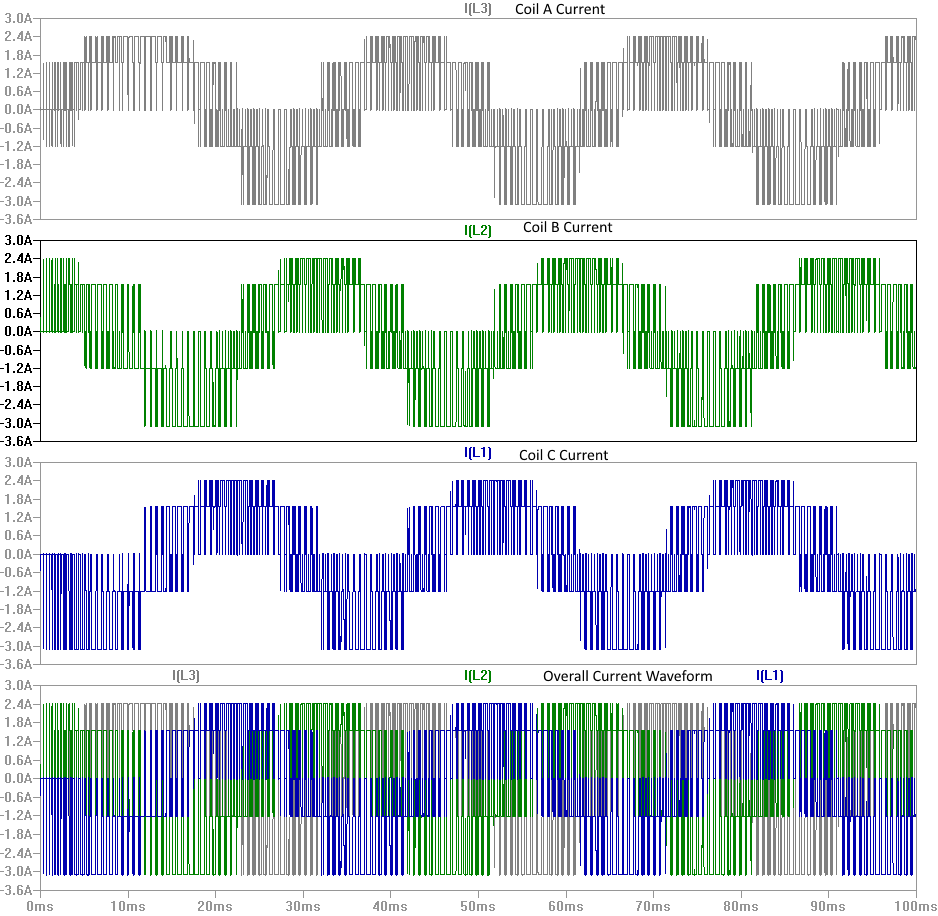
\includegraphics[scale=0.56,origin=c]{Motor_OUTPUT_AC.png}
\label{Triangle_Gen_Output}
\end{figure}

From the figure it is clear that the motor is achieving commutation through the required waveform cycling which approximates a sinusoidal waveform (hence sinewave pulse width modulation). Although not immediately evident in the figure it is assured that shorting of the H-bridge is impossible since the relevant control signals on each transistor pair are inverses as generated in the previous stage.

\section{Materials List}

\begin{figure}[H]
\centering
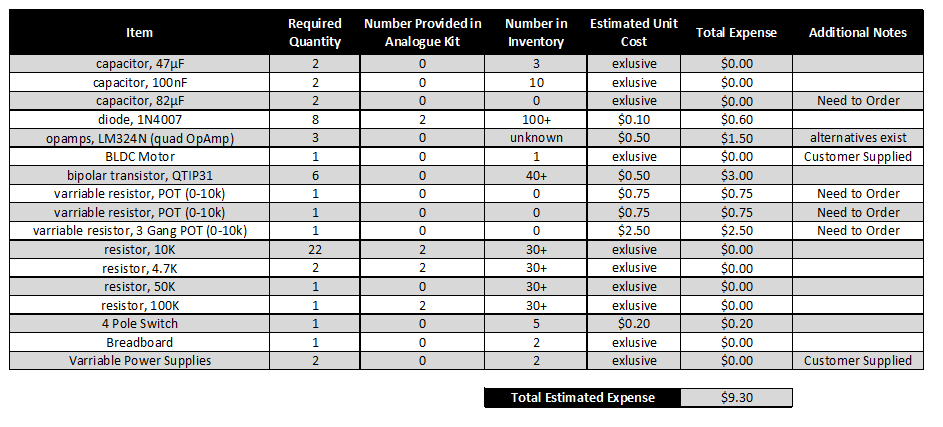
\includegraphics[scale=0.7,angle=90,origin=c]{Budget.png}
\label{Triangle_Gen_Output}
\end{figure}
\end{appendices}

\begin{thebibliography}{99}
	\bibitem{textbook}
	    A. Sedra, K. Smith. \emph{Microelectronic Circuits}. 7th ed.
	    New York: Oxford University Press, Nov. 2014.
	\bibitem{Notes}
		Freescale Semiconductor Ltd, \emph{Sensorless BLDC Motor Control Using MC9S08AW60}.
		DRM086,
		Rev. 0.1,
		January, 2007.
	\bibitem{Notes}
		Wilson, Dave. \emph{So, Which PWM Technique is Best}.
		Texas Instruments Motor Drive \& Control Blog,
		April, 2012.
	\bibitem{Notes}
		Yaskawa Electric America Inc, \emph{Variable Frequency Drives 3-Phase Motor Control}.
		AR.AFD.01,
		October, 2006.
	    
	    
\end{thebibliography}


\end{document}